%\cappos{Should I really just be using a hash here for integrity?   It's a 
%minor security loss and may really help with usability...}


\section{PolyPasswordHasher: Password Vertification}

This section describes one possible use of PolyHashing,
protecting password data stored on disk.   The resulting system is called
PolyPasswordHasher.
For ease of explanation, we describe PolyPasswordHasher using the hashing function
(SHA256) and threshold cryptography (Shamir Secret Sharing) used in its
implementation.
Passwords may only be checked by PolyPasswordHasher if a threshold of correct
passwords are known.   After describing the core algorithm for achieving
this, this section discusses domain specific extensions to this technique
that handle thresholdless passwords (those which do not count toward
the threshold) and alternative authentication mechanisms, such
as private key authentication, biometrics, and single sign-in systems.



\subsection{Core PolyPasswordHasher Algorithm}

Much like other password storage schemes, PolyPasswordHasher stores password data 
to allow users to login using a username and password.   However, unlike 
other schemes, if the encrypted password file is stolen, the users' passwords
are safe and cannot be individually cracked unless at least a threshold
of them are known.   This is true even if all data stored on disk is stolen
by an attacker.

With PolyPasswordHasher, a PolyHashing store is created to store user login data.
PolyPasswordHasher makes a few minor additions to the default PolyHashing scheme
(top half of Figure~\ref{fig-polypasswordhasheroverview}).   First of all, similar
to popular login systems, the store is keyed by username.   The corresponding
share number (that the index above derives) is stored explicitly in the 
database.   In this way, if an entry in the database is deleted or added, the
username to share number mapping remains to allow recovery.   Since
the set of used passwords is quite small and predictable, we use a 
salt~\cite{klein1990foiling}.

When a system using a PolyPasswordHasher store restarts, no authentication can
be performed.   First an initial threshold of passwords must be provided
before any can be checked.   When the system restarts, a set of users 
will try to authenticate in a normal way.   
%some subset of a set of administrators) can enter their passwords.
%(Alternatively, for a server in an office such as a mail server, the normal 
%flow of user requests may provide an adequate number of valid logins in a 
%short period of time.)   
When
sufficiently many correct passwords are obtained (discussed below), the server 
can reconstruct the random coefficients and authenticate users.
Once the initial set of correct authentications are performed, all subsequent
authentications are fast and efficient.

\subsubsection{What Is Stored}

As the top half of Figure~\ref{fig-polypasswordhasheroverview} shows, the server 
stores a file (or database) that contains records of the form:
$<$username, salt, sharenumber, (share XOR hash)$>$.   As may be 
expected, the username is the user's login.   The username, salt, and 
sharenumber
will all be known to an attacker that steals the database.   However,
as with PolyHashing, the share and hash are effectively random 
unless a threshold of shares (and thus hashes of passwords) are
known.

Note that the random coefficients for Shamir are private and are not stored on 
disk.   They are instead reconstructed in memory through Lagrange 
interpolation assuming an adequate number of shares are known.

\begin{figure}
\center
% We need pdflatex with png images. Plain latex would fail here.
% So, we conditionally include this so we can still build with latex,
% just without this image.
\begin{minipage}[b]{1.05\linewidth}
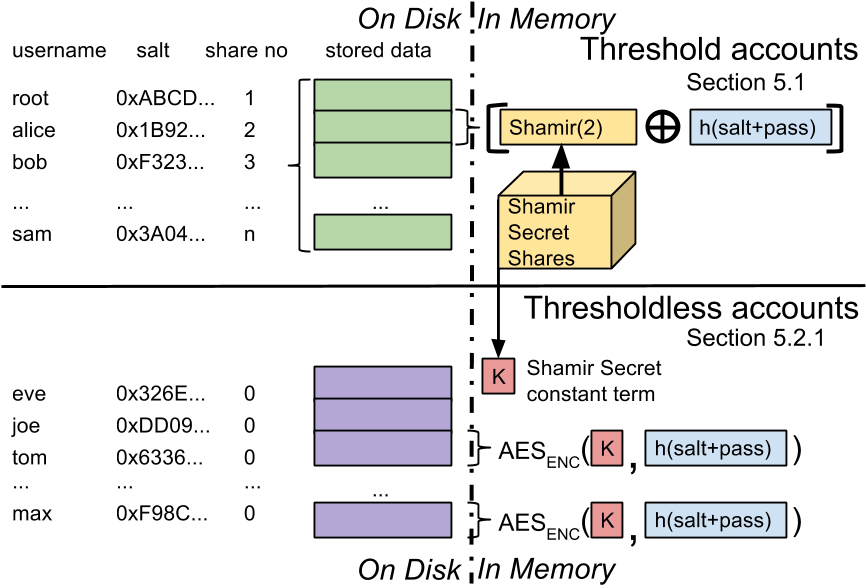
\includegraphics[width=\columnwidth]{figures/polypasswordhasheroverview.png}
\end{minipage}
\caption{The top portion of this figure demonstrates the data stored
by the basic PolyPasswordHasher algorithm.   The bottom portion shows how
thresholdless accounts have the salted hash of their password
encrypted by an AES key.   This AES key is stored as the secret for the 
threshold accounts and can only be recovered by the system if a threshold
of administrator passwords is known.}
\label{fig-polypasswordhasheroverview}
\end{figure}


\subsubsection{Checking A Password}

Assuming the server has enough valid passwords (and thus shares), the server 
can thus recover all shares.
The server computes the salted hash of the user's password and
XORs it with the last entry from the table (share XOR hash) to obtain 
the share.   If the share is valid, the password is correct.   The share will
consist of a set of $x$ values and $f(x)$ results.   To compute validity, 
one can evaluate $f(x)$ at the respective values and check to see if they
match.

Note that, a single account could optionally provide access 
to multiple shares.
To do this, there can be several entries with the same username that unlock 
using the same password, however each entry will have a different
salt and share number which leads to different stored data.   In this
case, the same password is hashed with different salt
and share numbers which effectively re-randomizes each component of
the stored data.

\subsubsection{Creating An Account}


As is shown in the top half of Figure~\ref{fig-polypasswordhasheroverview}, 
to add an account entry, one must have four items: username, salt, share
number, and stored data.   The server
randomly generates a salt, chooses an
unused share number, and uses the password's hash and share to
compute the shared data.   For example, if a user {\tt alice} needs an
account, the system will find an unused share number, such as 2 in the
above example.   Then the system computes a random salt, prepends
it to {\tt alice}'s password and computes the hash of this value.
This hash is XORed with the Shamir Secret Share's share number 2 and is stored
as the fourth field of the PolyPasswordHasher store.   The username, salt, share
number, and stored data are written to the PolyPasswordHasher store.


\subsubsection{Changing A Password}

Changing a password is a simple process for an unlocked store.  
Optionally, the procedure for account change may require validating the 
existing password first before allowing replacement.  The remaining steps 
required to change a password are nearly identical to account creation.  
The actual password change simply 
involves creating a new entry with the same username and sharenumber, but 
a different salt.  Since the salt and password have changed, the final
field will also change.   Once the new password entry is computed, it 
can replace the old one.   

If the PolyPasswordHasher database is also likely to be compromised, then it 
makes sense to additionally change the cryptosystem's secret information.
The reason is as follows.   Suppose an attacker compromises the password 
database repeatedly and knows the password for different accounts over a 
period of time.   From this information, the attacker may be able to recover 
enough shares from the
cryptosystem even if those accounts were not active at the same time.   To
combat this, one can easily change the cryptosystem's source of randomness
by computing a new random cryptosystem and XORing both the old and new 
shares with each stored data entry.   This effectively removes the prior
cryptosystem data while simultaneously adding randomness from the new
cryptosystem.   In this case, no user passwords are changed, so this
operation is not visible to the users in any way.


\subsubsection{Unlocking a PolyPasswordHasher Store}

To recover the random coefficients, the server takes a series of logins that 
have more than the threshold number of entries.   
%In fact, the server can (and should) check
%more than the threshold number of shares to validate the store is correctly
%unlocked.  
The server can either batch login requests and issue them all at once to
achieve this or simply wait for administrators with a sufficient threshold to 
attempt to login.   Then the password hashes are computed and the shares
are recovered.   Assuming that the provided information is valid, the 
cryptosystem will be able to use a technique like Lagrange interpolation to
recover all shares.

If more than the threshold number of shares are provided and some may be
invalid, individual user accounts (which may have 
incorrect logins) can be removed from the threshold to test their validity
so long as at least $k$ entries are validated.   %PolyPasswordHasher can leverage
%substantial prior work that detects and recovers from incorrect 
%shares~\cite{carpentieri1995perfect,Yang_compsac_02,devet2012optimally} in 
%threshold cryptosystems to find a valid set of entries.   
Furthermore, 
Section~\ref{sec-partial} describes an extension to partially validate 
passwords and discard a large percentage of incorrect values even before 
the threshold is reached.


